\documentclass[UTF-8,twoside,cs4size]{ctexart}
\usepackage{amsmath}
\usepackage{amssymb}
\usepackage{geometry}
\usepackage{setspace}
\usepackage{xeCJK}
\usepackage{ulem}
\usepackage{pstricks}
\usepackage{pstricks-add}
\usepackage{bm}
\usepackage{mathtools}
\usepackage{breqn}
\usepackage{mathrsfs}
\usepackage{esint}
\usepackage{textcomp}
\usepackage{upgreek}
\usepackage{pifont}
\usepackage{tikz}
\usepackage{circuitikz}
\usepackage{caption}
\usepackage{xcolor}
\usepackage{tabularx}
\usepackage{array}
\usepackage{pgfplots}
\usepackage{multirow}
\usepackage{pgfplotstable}

\newcolumntype{Y}{>{\centering\arraybackslash}X}
\geometry{a4paper,centering,top=0.75cm,bottom=2.54cm,left=2cm,right=2cm}
\pagestyle{plain}
\captionsetup{font=small}

\CTEXsetup[name={,.}]{section}
\CTEXsetup[format={\raggedright\bfseries\noindent\zihao{3}}]{section}
\CTEXsetup[format={\raggedright\bfseries\quad\large}]{subsection}
\CTEXsetup[format={\raggedright\bfseries\qquad}]{subsubsection}
\renewcommand\thefootnote{\ding{\numexpr171+\value{footnote}}}

\setstretch{1.5}

\setCJKfamilyfont{boldsong}[AutoFakeBold = {2.17}]{SimSun}
\newcommand*{\boldsong}{\CJKfamily{boldsong}}
%\DeclareMathOperator\dif{d\!}
\newcommand*{\me}{\mathop{}\!\mathrm{e}}
\newcommand*{\mpar}{\mathop{}\!\partial}
\newcommand*{\dif}{\mathop{}\!\mathrm{d}}
\newcommand*{\tab}{\indent}

\begin{document}
	\begin{flushright}
		\zihao{2}{分组号:3-07}
	\end{flushright}
	
	\noindent{\zihao{-2}\boldsong\bfseries 《\,\, 基\,\, 础\,\, 物\,\, 理\,\, 实\,\, 验\,\, 》\,\, 实\,\, 验\,\, 报\,\, 告\,\, }
	
	\noindent\textit{实验名称\uline{\quad\qquad\qquad\qquad 测量金属的杨氏模量\,\qquad\qquad\qquad\qquad}指导教师\uline{\qquad\,\,\,张易\quad\,\,\,\qquad}}
	
	\noindent\textit{姓\qquad 名\uline{\,\,\, 桂庭辉\,\,\,}\,学号\uline{\,\,\,{\upshape2019K8009929019}\,\,\,}\,专\qquad 业\uline{\,\,\,计算机科学与技术\,\,\,}\,班级\uline{\,\,\,\upshape{03}\,\,\,}\,座号\uline{\,\,\,\upshape{6}\,\,\,}}
	
	\noindent\textit{实验日期\uline{\,\,{\upshape 2020}\,\,}年\uline{\,\,{\upshape 11}\,\,}月\uline{\,\,{\upshape25}\,\,}日\,\,实验地点\uline{\,\,\,教学楼{\upshape710}\,\,\,}调课/补课\uline{\,\,\,$ \square $是\,\,\,}成绩评定\uline{\,\,\,\quad\qquad\qquad}}
	
	\begin{table}[h]
		\centering
		\psset{linewidth=2pt}
		\begin{pspicture}(-1,-0.1)(1,0.1)
		\psline(-9,0)(9,0)
		\end{pspicture}
	\end{table}

	\begin{center}
		\Large\bfseries 第一部分\quad 拉伸法测量金属的杨氏模量
	\end{center}

	\section{实验目的}
	1.学会用CCD\footnote{Charge Coupled Device,电荷耦合器件}杨氏模量测量仪测量长度的微小变化量;
	
	2.学会测定金属丝杨氏弹性模量的一种方法;
	
	3.学习用逐差法、作图法和最小二乘法处理数据;
	
	4.学会不确定的计算方法,结果的正确表达。
	
	\section{实验仪器与用具}
	CCD杨氏弹性模量测量仪、螺旋测微器、钢卷尺。
	
	\textit{{\upshape CCD}杨氏弹性模量测量仪的主要技术指标有};
	
	\tab\tab 1.\textit{采用分划板{\upshape +\,CCD}测量显微镜系统$ + $彩色液晶监视器方案;}
	
	\tab\tab 2.\textit{立柱:不锈钢双柱高约$ 85\,\mathrm{cm} $};
	
	\tab\tab 3.\textit{钼丝:长约$ 60\,\mathrm{cm} $,直径$ 0.18\,\mathrm{mm} $,悬挂位置及长度可调节};
	
	\tab\tab 4.\textit{监视器:彩色液晶监视器};
	
	\tab\tab 5.\textit{分化板:刻度范围$ 4\,\mathrm{mm} $,分度值$ 0.05\,\mathrm{mm} $,设有限位槽,可防止来回摆动,采用{\upshape LED}照明};
	
	\tab\tab 6.\textit{{\upshape CCD}测量显微镜系统:放大倍率$ 60 $倍,内含电子刻度线,可二维调节,可卸下用于其他微位移测量场合,采用高级面阵{\upshape CCD},信噪比$ \geq 52\,\mathrm{db} $,分辨率$ 480\,\mathrm{TVL} $,视频输出幅度:$ 1.0\,\mathrm{V_{P-P}}/75\,\Omega $};
	
	\tab\tab 7.\textit{砝码组:$ 10 $个砝码,$ 200 $克$ 8 $个及$ 100 $克$ 2 $个};
	
	\tab\tab 8.\textit{底座沉稳,可进行水平调节,设有储藏格可贮存砝码组};
	
	\tab\tab 9.\textit{测量相对不确定度:$ <5\% $}.
	
	\newpage
	
	\section{实验原理}
	物体在外力作用下都会发生形变。当形变不超过某一限度时,撤走外力之后,形变消失,物体形状恢复原状态,这样的形变称为弹性形变。弹性形变发生时,物体内部会产生恢复原状的内应力。弹簧模量即为反映材料形变与内应力关系的物理量。
	
	\subsection{杨氏模量}
	记柱状物体的长度为$ L $,截面积为$ S $,沿长度方向受外力$ F $作用后伸长(或缩短)$ \Delta L $,单位横截面积上垂直作用力$ \frac FS $称为正应力,物体的相对伸长$ \frac{\Delta L}{L} $称为线应变。在弹性范围内,正应力与线应变成正比,即
	\[\frac FS=Y\frac{\Delta L}{L}\]
	该规律称为虎克定律。式中比例系数$ Y $即为杨氏弹性模量,其单位为$ \mathrm{N/m^2} $,其完全由材料的性质决定,与材料的几何形状无关。
	
	本实验中测量钼丝的杨氏弹性模量,实验方法为将钼丝悬挂在支架上,上端固定,下端通过加砝码对钼丝施加力$ F $(由砝码的质量求出),测出钼丝相应的伸长量$ \Delta L $,用钢卷尺测出钼丝长度$ L $,用螺旋测微器测处钼丝直径$ d $,则可求得钼丝横截面积$ S=\frac{\pi d^2}{4} $。那么根据虎克定律可知
	\[Y=\frac{4FL}{\pi d^2\Delta L}\]
	
	\subsection{测量原理}
	实际测量过程中,钼丝的伸长量很小,约为$ 10^{-1}\,\mathrm{mm} $数量级。所以本次实验中$ \Delta L $的测量采用显微镜和CCD成像系统进行测量。钼丝下端加上一定质量的砝码时,十字叉丝随着金属丝的伸长同样下降$ \Delta L $,而叉丝板通过显微镜的物镜成像在最小分度为$ 0.05\,\mathrm{mm} $的分划板上,CCD摄像机的镜头将显微镜的光学图象汇聚到CCD上,再变成视频电信号,经视频电缆传送到显示器上,供实验者读取。
	
	\section{实验内容}
	\subsection{注意事项}
	1.使用CCD摄像机时不能将CCD器件正对太阳、激光或其他强光源,注意保护镜头,如非特别需要不要随意卸下。
	
	2.钼丝必须保持直线形态。测量直径时需要特别谨慎,避免扭转、拉扯、牵挂钼丝导致其折弯变形。
	
	3.读数时需等到刻度值稳定后才能进行读数。
	
	4.将砝码放置于砝码盘的时候需保证轻拿轻放,防止钼丝突然受力而断裂。
	\subsection{调节仪器}
	用螺旋底角调平底座,使叉丝组分划板正对CCD摄像头。调节下横梁高度,保证叉丝组放置在下横梁的槽内。将CCD摄像头与分划板放置在同一水平面上,调节CCD摄像头位置,直到可以观察到清晰的像且分划板刻度尺的像在监视器的中心。
	\subsection{测量数据}
	(1)在测量钼丝杨氏模量前,先放2块100\,g的砝码把钼丝拉直,保证分划板在下横梁槽内,避免在拉直过程中分划板的旋转。
	
	(2)记下待测细丝下的砝码盘中仅有已加的2块100\,g砝码时屏幕上显示的毫米尺在横线上的读数$ l_0 $,然后再砝码上依次加上8个$ M=200\,\mathrm{g} $的砝码,记下相应的叉丝读数$ l_i\;(i=1,2,\cdots,8) $。然后逐一减掉砝码,再读取$ l_8',l_7',\cdots,l_1' $。此过程中需注意轻拿轻放砝码,避免因增减砝码使得砝码盘产生微小振动而使得读数起伏较大。
	
	(3)取同一符合下叉丝读数的平均值$ \bar l_1,\bar l_2,\cdots,\bar l_8 $,用逐差法求出钼丝荷重增减四个砝码时光标的平均偏移量$ \Delta l $。
	
	(4)用钢卷尺测量上下夹头之间的钼丝长度$ L $。
	
	(5)用螺旋测微器测量钼丝直径$ d $,由于钼丝直径可能不均匀,需再上、中、下各部进行测量,每个位置在相互垂直的方向各测一次。
	
	(6)将前述原理公式整理可得
	\begin{equation}\label{1-Yang}
		Y=\frac{4MgL}{\pi d^2\Delta l}
	\end{equation}
	式中$ \Delta l $与$ M $有对应关系,本实验中$ \Delta l $是荷重增减4个砝码所引起的光标偏移量,则$ M $为4个砝码的质量。
	
	~\\
	
	\section{实验结果与数据处理}
	\subsection{数据记录}
	1.钼丝长度$ L=578.9\,\mathrm{mm} $,其不确定度为$ u(L)=\sqrt{\frac{d^2}{10^2}+\frac{e^2}{3}}=1.159\,\mathrm{mm} $.
	
	2.钼丝直径测得的数据记录如表(1).
	\begin{table}[!h]
		\centering
		\renewcommand\arraystretch{1.5}
		\begin{tabularx}{\textwidth}{|c|Y|Y|Y|Y|Y|Y|c|}
			\hline
			\textbf{测量次数}&\textbf{1}&\textbf{2}&\textbf{3}&\textbf{4}&\textbf{5}&\textbf{6}&\textbf{平均值$ \bm{\bar d} $}\\
			\hline
			$ \bm{d\,(\mathbf{mm})} $ &0.178&0.180&0.170&0.176&0.180&0.176&0.1767\\
			\hline
		\end{tabularx}
		\caption{钼丝直径测量数据}
	\end{table}

	其不确定度为$ u(d)=\sqrt{\frac{\sum_{i=1}^6(x_i-\bar x)^2}{6^2-6}+\frac{e^2}{3}}=0.0028\,\mathrm{mm} $.(估读所用最小精度为$ \frac{d}{10} $)
	
	3.(此处读数估读所用最小精度为$ \frac d5 $)实验过程中加上两个100\,g砝码作为底码后,初始读数为$ l_0=1.05\,\mathrm{mm} $,此后累加与累减8个200\,g砝码时记录叉丝读数如下:
	\begin{table}[!h]
		\centering
		\renewcommand\arraystretch{1.5}
		\begin{tabularx}{\textwidth}{|c|Y|Y|Y|c|}
			\hline
			\textbf{砝码质量$ \bm M $(g)}&\textbf{加载$ \bm{l_i} $(mm)}&\textbf{卸载$ \bm{l_i'} $(mm)}&\textbf{平均值$ \bm{\bar l_i} $(mm)}&$ \bm{l_iM_i} $\textbf{(mm$ \bm\cdot $g)}\\
			\hline
			\textbf{200}&1.22&1.24&1.23&246.0\\
			\hline
			\textbf{400}&1.41&1.48&1.445&578.0\\
			\hline
			\textbf{600}&1.62&1.62&1.62&972.0\\
			\hline
			\textbf{800}&1.80&1.84&1.82&1456.0\\
			\hline
			\textbf{1000}&1.97&2.00&1.985&1985.0\\
			\hline
			\textbf{1200}&2.16&2.20&2.18&2616.0\\
			\hline
			\textbf{1400}&2.34&2.36&2.35&3290.0\\
			\hline
			\textbf{1600}&2.52&2.52&2.52&4032.0\\
			\hline
		\end{tabularx}
	\\
		\begin{tabularx}{\textwidth}{|Y|Y|Y|Y|c|Y|}
			\hline
			$ \sum M\;(\mathrm g) $&$ \overline M\;(\mathrm g) $&$ \sum\bar l\;(\mathrm{mm}) $&$ \bar{\bar l}\;(\mathrm{mm}) $&$ \sum l_iM_i\;(\mathrm{mm\cdot g}) $&$ \overline{l_iM_i}\;(\mathrm{mm\cdot g}) $\\
			\hline
			7200&900&15.15&1.89375&15175&1896.875\\
			\hline
		\end{tabularx}
		\caption{增减砝码时叉丝读数数据记录}
		\label{tab1-2}
	\end{table}

	\subsection{逐差法处理数据}

	根据逐差法计算增减四个200\,g砝码时引起的长度变化为
	\[\overline{\Delta\bar l}=\sum_{i=1}^4\frac{\bar l_{i+4}-\bar l_i}{4}=\frac{(1.985-1.23)+(2.18-1.445)+(2.35-1.62)+(2.52-1.82)}{4}\,\mathrm{mm}=0.73\,\mathrm{mm}\]
	其不确定度为
	\(u(\Delta\bar l)=\sqrt{\frac{d^2}{5^2}+\frac{d^2}{5^2}+\frac{e^2}{3}}=0.0144\,\mathrm{mm}\)
	
	取$ g=9.8\,\mathrm{m/s^2} $,并将其他测得的物理量:$ m=0.8\,\mathrm{kg},\;L=578.9\,\mathrm{mm},\;d=0.1767\,\mathrm{mm} $代入杨氏模量计算公式(\ref{1-Yang})计算得到
	\[Y=\frac{4MgL}{\pi d^2\Delta l}=2.535\times10^{11}\,\mathrm{N/m^2}\]
	根据此前已计算得到的各不确定度可求得
	\[u(Y)=Y\sqrt{\frac{u^2(L)}{L^2}+\frac{u^2(d)}{d^2}+\frac{u^2(\Delta\bar l)}{(\Delta\bar l)^2}}=0.064\times10^{11}\,\mathrm{N/m^2}\]
	所以最终结果为
	\[Y=(2.535\pm 0.064)\times10^{11}\,\mathrm{N/m^2}\]
	与标准值间的相对误差为$ 10.22\% $.
	
	\subsection{最小二乘法处理数据}
	
	可将式(\ref{1-Yang})改写为
	\[\Delta l=\frac{4gL}{\pi d^2Y}m\]
	记斜率为$ k=\frac{4gL}{\pi d^2Y} $,根据表(\ref{tab1-2})中数据用最小二乘法可求得斜率
	\[k=\frac{\overline{m_i\bar l_i}-\overline m_i\bar{\bar l}_i}{\overline{m_i^2}-\overline m_i^2}=9.17\times10^{-4}\,\mathrm{mm/g}\]
	故而可计算求得
	\[Y=\frac{4gL}{\pi d^2k}=2.523\times10^{11}\,\mathrm{N/m^2}\]
	与理论值的相对误差为9.70\%.
	
	\subsection{作图法处理数据}
	根据表(\ref{tab1-2})中数据可如下拟合图象:
	
	\begin{figure}[!h]
		\centering
		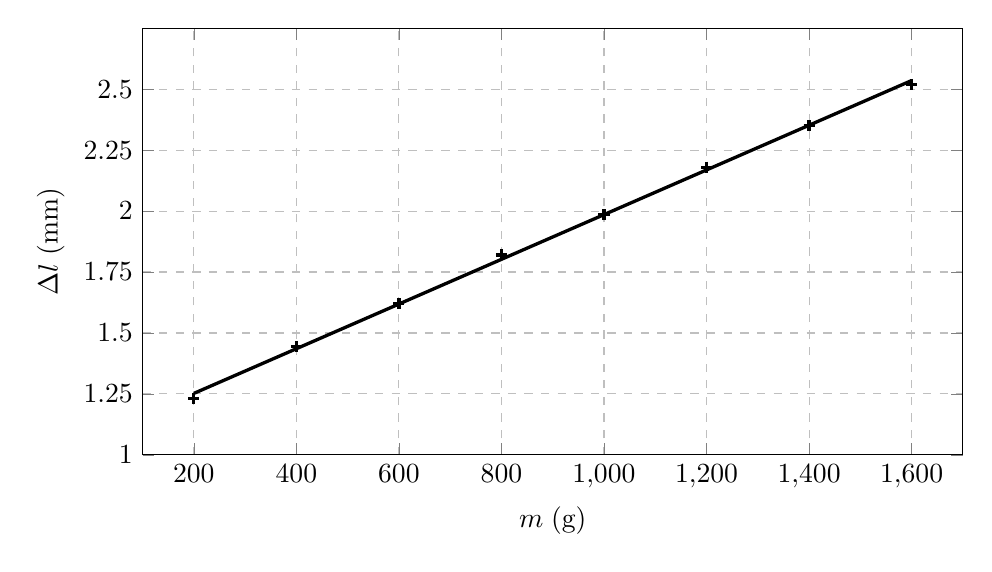
\begin{tikzpicture}
			\begin{axis}[
				%legend pos=outer north east,
				width=12cm,height=7cm,
				xlabel=$ m\;(\mathrm{g}) $,
				ylabel=$ \Delta l\;(\mathrm{mm}) $,
				xmin=100,xmax=1700,
				ymin=1,ymax=2.75,
				xtick={200,400,600,800,1000,1200,1400,1600},
				ytick={1.0,1.25,1.5,1.75,2,2.25,2.5},
				grid style=dashed,
				ymajorgrids=true,
				xmajorgrids=true,
				]
				\addplot[no marks,black,very thick] table[y={create col/linear regression={y=Y}}]
				{
					X	Y
					200	1.23
					400	1.445
					600 1.62
					800	1.82
					1000	1.985
					1200	2.18
					1400	2.35
					1600	2.52				
				};
				%\addlegendentry{
				%	$\pgfmathprintnumber{\pgfplotstableregressiona} \cdot x
				%	\pgfmathprintnumber[print sign]{\pgfplotstableregressionb}$}
				
				\addplot [very thick,mark=+,only marks] coordinates {
					(200,1.23)(400,1.445)(600,1.62)(800,1.82)
					(1000,1.985)(1200,2.18)(1400,2.35)(1600,2.52)
				};
			\end{axis}
		\end{tikzpicture}
		\caption{作图法求杨氏模量}
	\end{figure}
	取直线上较远两点算得斜率$ k=9.22\times10^{-4}\,\mathrm{mm/g} $,故而可计算求得
	\[Y=\frac{4gL}{\pi d^2k}=2.537\times10^{11}\,\mathrm{N/m^2}\]
	与理论值的相对误差为10.30\%.
	\newpage
	
	~\
	
	\begin{center}
		\Large\bfseries 第二部分\quad 霍尔位置传感方法测量杨氏模量
	\end{center}
	\setcounter{section}{0}
	
	\section{实验目的}
	1.熟悉霍尔位置传感器的特性;
	
	2.弯曲法测量黄铜的杨氏模量;
	
	3.测黄铜的杨氏模量的同时,对霍尔位置传感器定标;
		
	\section{实验器材}
	霍尔位置传感器测杨氏模量实验装置一台、霍尔位置传感器测杨氏模量测试仪一台、游标卡尺、螺旋测微器、钢卷尺。
	
	{\kaishu 实验仪器的主要技术指标有:}
	
	{\kaishu 1.读数显微镜:目镜放大率10倍,目镜测微鼓轮最小分度值0.01\,mm,物镜放大率2倍,测量范围为$ 0\sim 6\,\mathrm{mm} $,鼓轮实际读数最小分辨率0.005\,mm。}
	
	{\kaishu 2.电子传感器加力系统:$ 0\sim 199.9\,\mathrm{g} $连续可调,三位半数显。}
	
	{\kaishu 3.霍尔电压表有两档量程:量程1为$ 0\sim 199.9\,\mathrm{mV} $,分辨率$ 0.1\,\mathrm{mV} $;量程2为$ 0\sim 1.999\,\mathrm{V} $,分辨率$ 1\,\mathrm{mV} $。}
	
	{\kaishu 4.霍尔位置传感器:灵敏度大于$ 250\,\mathrm{mV/mm} $,线性范围$ 0\sim 2\,\mathrm{mm} $。}
	
	\section{实验原理}
	
	\subsection{霍尔位置传感器的定标}
	霍尔元件置于磁感强度为$ B $的磁场中,再垂直于磁场的方向上加上电流$ I $,那么在与这两者垂直的方向上将产生霍尔电势差
	\[U_H=K\cdot I\cdot B\]
	其中$ K $为元件的霍尔灵敏度。若保持霍尔元件的电流$ I $不变,而使其在一个均匀梯度的磁场中移动时,输出的霍尔电势差变化量为
	\[\Delta U_H=K\cdot I\cdot\frac{\dif B}{\dif Z}\cdot\Delta Z\]
	上式中$ \Delta Z $为位移量。
	
	\begin{figure}[!h]
		\centering
		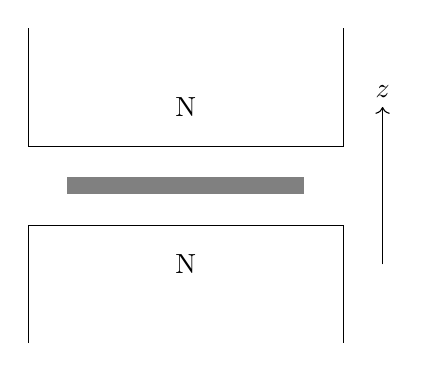
\begin{tikzpicture}
			\filldraw[gray] (-1.5,-0.1) rectangle (1.5,0.1);
			\draw (-2,2)--(-2,0.5)--(2,0.5)--(2,2);
			\draw (-2,-2)--(-2,-0.5)--(2,-0.5)--(2,-2);
			\draw[->] (2.5,-1)--(2.5,1) node[above] {$ z $};
			\node at(0,1) {N};
			\node at(0,-1) {N};
		\end{tikzpicture}
		\caption{梯度均匀磁场的实现}
	\end{figure}
	为实现均匀梯度的磁场,可以如上图所示将两块相同\footnote{磁铁截面积及表面感应强度相同}的磁铁N极与N极相对,两磁铁间留一等间距间隙。霍尔元件垂直于$ z $轴放置于该间隙的中轴上。间隙大小根据测量范围和测量灵敏度要求而定:间隙越小,磁场梯度越大,灵敏度越高。此外为减小边缘效应的影响,磁铁截面需远大于霍尔元件。
	
	若磁铁间隙内中心截面处的磁感应强度为0,那么霍尔元件于该处输出的霍尔电势差应该为0。当霍尔元件偏离中心沿$ z $轴发生位移时,由于磁感应强度不再为0,霍尔元件随之产生相应的电势差输出,由电压表可测得其大小。故而可将霍尔电势差为0时元件位置作为位移参考零点。
	
	霍尔电势差与位移量间存在一一对应关系,当位移量较小($ <2\,\mathrm{mm} $)时,该对应关系具有良好的线性。
	
	\subsection{弯曲法测杨氏模量}
	如下图所示,设金属篇在刀口间的长度为$ d $,金属片的厚度为$ a $,宽度为$ b $。
	\begin{figure}[!h]
		\centering
		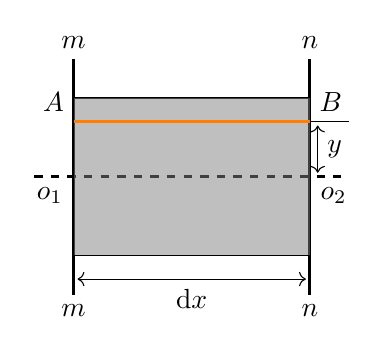
\begin{tikzpicture}
			\draw[dashed,very thick] (-2,0)--(-1.5,0) node[below left]{$ o_1 $}--(1.5,0) node[below right]{$ o_2 $}--(2,0);
			\draw[very thick] (-1.5,-1.5)--(-1.5,1.5);
			\draw[very thick] (1.5,-1.5)--(1.5,1.5);
			\draw (-1.5,-1)--(1.5,-1);
			\draw (-1.5,1)--(1.5,1);
			\fill[gray,fill opacity=0.5] (-1.5,-1) rectangle (1.5,1);
			\draw[<->] (-1.45,-1.3)--(1.45,-1.3);
			\node[below] at(0,-1.3) {$ \dif x $};
			\node[below] at(-1.5,-1.5) {$ m $};
			\node[below] at(1.5,-1.5) {$ n $};
			\node[above] at(-1.5,1.5) {$ m $};
			\node[above] at(1.5,1.5) {$ n $};
			\draw[very thick,orange] (-1.5,0.7)--(1.5,0.7);
			\node[above left] at(-1.5,0.7) {$ A $};
			\node[above right] at(1.5,0.7) {$ B $};
			\draw (1.5,0.7)--(2,0.7);
			\draw[<->] (1.6,0.05)--(1.6,0.65);
			\node[right] at(1.6,0.35) {$ y $};
		\end{tikzpicture}
		\qquad\qquad
		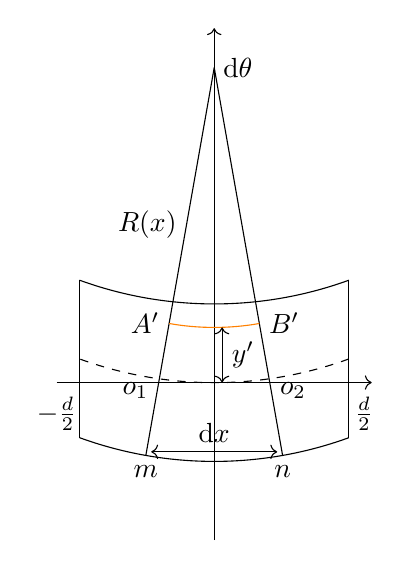
\begin{tikzpicture}
			\draw (1.71,0.3) arc (290:250:5);
			\draw (1.71,2.3) arc (290:250:5);
			%\draw (0,5)--(1,5);
			\draw (1.71,0.3)--(1.71,2.3);
			\draw (-1.71,0.3)--(-1.71,2.3);
			\draw (0.8682,0.0760)node[below]{$ n $} -- (0,5);
			\draw (-0.8682,0.0760)node[below]{$ m $} -- (0,5);
			\draw[->] (0,-1)--(0,5.5);
			\draw[->] (-2,1)--(2,1);
			\draw[dashed] (1.71,1.3) arc (290:250:5);
			\draw[<->] (-0.8,0.12)--node[above]{$ \dif x $} (0.8,0.12);
			\node at(1.9,0.6) {$ \frac d2 $};
			\node at(-2,0.6) {$ -\frac d2 $};
			\node at(-1,0.9) {$ o_1 $};
			\node at(1,0.9) {$ o_2 $};
			\node at(-0.85,3) {$ R(x) $};
			\node at(0.3,5) {$ \dif\theta $};
			\draw[orange] (0.573,1.7501) arc (280:260:3.3);
			\node[left] at(-0.573,1.7501) {$ A' $};
			\node[right] at(0.573,1.7501) {$ B' $};
			\draw[<->] (0.1,1)--node[right]{$ y' $} (0.1,1.7);
		\end{tikzpicture}
		\caption{弯曲法测杨氏模量原理示意图}
	\end{figure}

	$ o_1o_2 $所在平面为中性面,既不拉伸也不压缩,$ AB $为距中性面距离$ y $处的平面。变形前有$ o_1o_2=AB=\dif x $,变形后则为$ o_1o_2=\dif x=R(x)\dif\theta,\;A'B'=(R(x)-y)\dif\theta $.
	
	那么$ AB $面的应变为
	\[\varepsilon=\frac{A'B'-AB}{AB}=\frac{(R(x)-y)\dif\theta-\dif x}{\dif x}=\frac{(R(x)-y)\dfrac{\dif x}{R(x)}-\dif x}{\dif x}=-\frac{y}{R(x)}\]
	根据胡克定律$ \frac{\dif F}{\dif S}=Y\varepsilon=-Y\frac{y}{R(x)} $且$ \dif S=b\dif y $,因此有
	\[\dif F(x)=-\frac{Y\dif y}{R(x)}\dif y\]
	对中性面的转矩为
	\begin{equation}\label{2-1}
		\dif\mu(x)=|\dif F(x)|y=\frac{Yb}{R(x)}y^2\dif y
	\end{equation}
	积分可得
	\[\mu(x)=\int_{-a/2}^{a/2}\frac{Yb}{R(x)}y^2\dif y=\frac{Yba^3}{12R(x)}\]
	对梁上各点有$ \frac{1}{R(x)}=\frac{y''(x)}{[1+y'(x)]^{3/2}} $,由于梁的弯曲很小,$ y'(x)=0 $,所以
	\begin{equation}\label{2-2}
		R(x)=\frac{1}{y''(x)}
	\end{equation}
	在平衡时,梁在$ x $处的转矩应与梁右端支撑力$ \frac{Mg}{2} $对$ x $处的力矩平衡,因此有
	\begin{equation}\label{2-3}
		\mu(x)=\frac{Mg}{2}\left(\frac d2-x\right)
	\end{equation}
	由(\ref{2-1}),(\ref{2-2}),(\ref{2-3})可得
	\[y''(x)=\frac{6Mg}{Yba^3}\left(\frac d2-x\right)\]
	代入边界条件$ y(0)=0,\;y'(0)=0 $可求得
	\[y(x)=\frac{3Mg}{Yba^3}\left(\frac d2x^2-\frac13x^3\right)\]
	在中点$ x=\frac d2 $处,有
	\[\Delta z=y\left(\frac d2\right)=\frac{Mgd^3}{4Yba^3}\]
	所以杨氏模量为
	\begin{equation}\label{2}
		Y=\frac{d^3Mg}{4a^3b\Delta Z}
	\end{equation}
	其中$ d $为两刀口间的距离,$ M $为所加拉力对应的质量,$ a $为梁的厚度,$ b $为梁的宽度,$ \Delta Z $为梁中心由于外力作用而下降的距离,$ g $为重力加速度。
	
	\section{实验内容}
	\subsection{注意事项}
	1.使用千分尺测量黄铜厚度$ a $时,旋转千分尺至将要与金属接触时需用微调轮。听到三声“嗒”后停止旋转。
	
	2.读数显微镜的准线对准时需注意与铜刀口上的基线对准而非黄铜梁的边沿。
	
	3.霍尔位置传感器定标前,需先将霍尔位置传感器调整到零输出位置。
	
	4.实验完成后,需调节加力调节旋钮,使得加力为零。
	
	5.实验开始前需检查横梁是否弯曲,如有需矫正。
	
	6.加力旋钮旁的锁紧螺钉需松紧适度,在一次实验过程中,加力调节仅向加力方向调节,不可回调,一次实验完成后放松锁紧螺钉,用手助力使得拉力传感器恢复到初始位置。
	
	\subsection{实验步骤}
	1.调节使得霍尔位置传感器探测元件位于磁铁中间的位置。
	
	2.用水平泡观察平台是否处于水平位置,若偏离则调节水平调节机脚。
	
	3.通过磁体调节结构上下移动磁铁,当毫伏表读数很小时,停止调节并固定螺丝,最后调节电位器使得毫伏表读数为零。
	
	4.调节读数显微镜,使得眼睛观察十字线与分划板刻度线和数字清晰,移动读数显微镜前后距离,使得铜刀口上的基线清晰。转动读数显微镜读数鼓轮使得铜刀口上的基线与读数显微镜内十字刻度线吻合,记下初始读数值。
	
	5.在拉力绳不受力的情况下将电子秤传感器加力系统调零。
	
	6.通过加力调节旋钮以20\,g为步长逐次增加拉力,相应地从读数显微镜上读出梁的弯曲位移$ \Delta Z_i $,从霍尔数字电压表上读出相应的霍尔电压$ U_i $。
	
	7.测量试样在两刀口间的长度$ d $,不同位置横梁宽度$ b $以及横梁厚度$ a $。
	
	8.用逐差法处理数据并分析,求得黄铜材料的杨氏模量与霍尔位置传感器的灵敏度$ \frac{\Delta U_i}{\Delta Z_i} $。
	
	\section{实验结果与数据处理}
	\subsection{数据记录}
	1.测得黄铜横梁的几何尺寸如下
	\begin{table}[!h]
		\centering
		\renewcommand\arraystretch{1.15}
		\begin{tabularx}{\textwidth}{|c|Y|Y|Y|Y|Y|Y|Y|Y|c|}
			\hline
			\textbf{长度$ \bm d $/mm}&\multicolumn{8}{c|}{222.7}&\textbf{平均值}\\
			\hline
			\textbf{宽度$ \bm b $/mm}&\multicolumn{2}{c|}{22.40}&\multicolumn{2}{c|}{22.70}&\multicolumn{2}{c|}{23.05}&\multicolumn{2}{c|}{22.76}&22.7275\\
			\hline
			\textbf{厚度$ \bm a $/mm}&0.971&0.972&0.980&0.982&0.975&0.970&0.970&0.967&0.973375\\
			\hline
		\end{tabularx}
		\caption{黄铜横梁几何尺寸数据记录}		
	\end{table}

	其中各项的不确定度分别为
	\begin{gather}
		u(d)=\sqrt{\frac{d^2}{10^2}+\frac{e^2}{3}}=0.07\,\mathrm{mm},\\
		u(b)=\sqrt{\frac{\sum_{i=1}^4(b_i-\bar b)^2}{4(4-1)}+\frac{e^2}{3}}=0.1338\,\mathrm{mm},\\
		u(a)=\sqrt{\frac{\sum_{i=1}^8(a_i-\bar a)^2}{8(8-1)}+\frac{e^2}{3}}=0.0029\,\mathrm{mm}
	\end{gather}

	2.读数显微镜示数:初始读数$ Z_0=3.625\,\mathrm{mm} $,调节加力系统以20\,g为步长步进得到如下数据:
	\begin{table}[!h]
		\centering
		\renewcommand\arraystretch{1.5}
		\begin{tabularx}{\textwidth}{|c|Y|Y|Y|Y|Y|}
			\hline
			\textbf{序号$ \bm i $}&\textbf{1}&\textbf{2}&\textbf{3}&\textbf{4}&\textbf{5}\\
			\hline
			$ {M_i\;\mathrm{(g)}} $&20.8&41.0&60.5&80.6&100.5\\
			\hline
			$ {Z_i\;\mathrm{(mm)}} $&3.830&4.019&4.300&4.550&4.810\\
			\hline
			$ {U_i\;\mathrm{(mV)}} $&79.6&165.7&246&325&399\\
			\hline
			$ {Z_i^2\;\mathrm{(mm^2)}} $&14.669&16.152&18.490&20.703&23.136\\
			\hline
			$ U_i^2\;\mathrm{(mV^2)} $&6336.2&27456&60516&105625&159201\\
			\hline
			$ Z_iU_i\;\mathrm{(mm\cdot mV)} $&304.87&665.95&1057.80&1478.75&1919.19\\
			\hline
		\end{tabularx}
	\\
		\begin{tabularx}{\textwidth}{|c|Y|Y|Y|Y|}
			\hline
			\textbf{序号$ \bm i $}&\textbf{6}&\textbf{7}&\textbf{8}&\textbf{平均值}\\
			\hline
			$ {M_i\;\mathrm{(g)}} $&120.5&140.2&160.5&90.575\\
			\hline
			$ {Z_i\;\mathrm{(mm)}} $&5.045&5.285&5.560&4.675\\
			\hline
			$ {U_i\;\mathrm{(mV)}} $&477&549&619&357.538\\
			\hline
			$ {Z_i^2\;\mathrm{(mm^2)}} $&25.452&27.931&30.914&22.181\\
			\hline
			$ U_i^2\;\mathrm{(mV^2)} $&227529&301401&383161&158903.15\\
			\hline
			$ Z_iU_i\;\mathrm{(mm\cdot mV)} $&2046.47&2901.47&3441.64&1727.02\\
			\hline
		\end{tabularx}
	
	~\\
	
		\begin{tabularx}{\textwidth}{|c|Y|Y|Y|Y|Y|}
			\hline
			\textbf{序号$ \bm i $}&\textbf{1}&\textbf{2}&\textbf{3}&\textbf{4}&\textbf{平均值}\\
			\hline
			$ \Delta Z_i=Z_{i+4}-Z_i\;\mathrm{(mm)} $&0.980&1.026&0.985&1.010&1.000\\
			\hline
			$ \Delta U_i=U_{i+4}-U_i\;\mathrm{(mV)} $&319.4&311.3&303&294&306.9\\
			\hline
		\end{tabularx}
		\caption{读数显微镜与霍尔数字电压表示数记录}
		\label{tab2-2}
	\end{table}

	\subsection{逐差法求杨氏模量}
	逐差法求得的$ \overline{\Delta Z} $的不确定度为
	\[u(\Delta Z)=\sqrt{\frac{d^2}{10^2}+\frac{d^2}{10^2}+\frac{e^2}{3}}=0.0018\,\mathrm{mm}\]
	取重力加速度$ g=9.8\,\mathrm{m/s^2} $,将表(\ref{2-2})的数据代入弯曲法的杨氏模量计算公式得
	\[Y=\frac{d^3Mg}{4a^3b\Delta Z}=1.169\times10^{11}\,\mathrm{N/m^2}\]
	其不确定度为
	\[u(Y)=Y\sqrt{\frac{u^2(d)}{d^2}+\frac{u^2(a)}{a^2}+\frac{u^2(b)}{b^2}+\frac{u^2(\Delta Z)}{(\Delta Z)^2}}=0.008\times10^{11}\,\mathrm{N/m^2}\]
	所以最终测量结果为$ Y=(1.169\pm 0.008)\times10^{11}\,\mathrm{N/m^2} $,与理论值$ 1.06\times10^{11}\,\mathrm{N/m^2} $的相对误差大小为$ 10.28\% $.
	
	\subsection{计算霍尔位置传感器的灵敏度系数}
	\textbf{(1)逐差法:}
	\[KI\frac{\dif B}{\dif Z}=\frac{\Delta U_i}{\Delta Z_i}=306.90\,\mathrm{mV/mm}\]
	
	\textbf{(2)最小二乘法}
	\[KI\frac{\dif B}{\dif Z}=\frac{\Delta U}{\Delta Z}=\frac{\overline{ZU}-\bar Z\bar U}{\overline{Z^2}-(\bar Z)^2}=308.14\,\mathrm{mV/mm}\]
	
	\textbf{(3)作图法}
	
	根据表(\ref{tab2-2})中数据可作出如下$ U-Z $图象:
	\begin{figure}[!h]
		\centering
		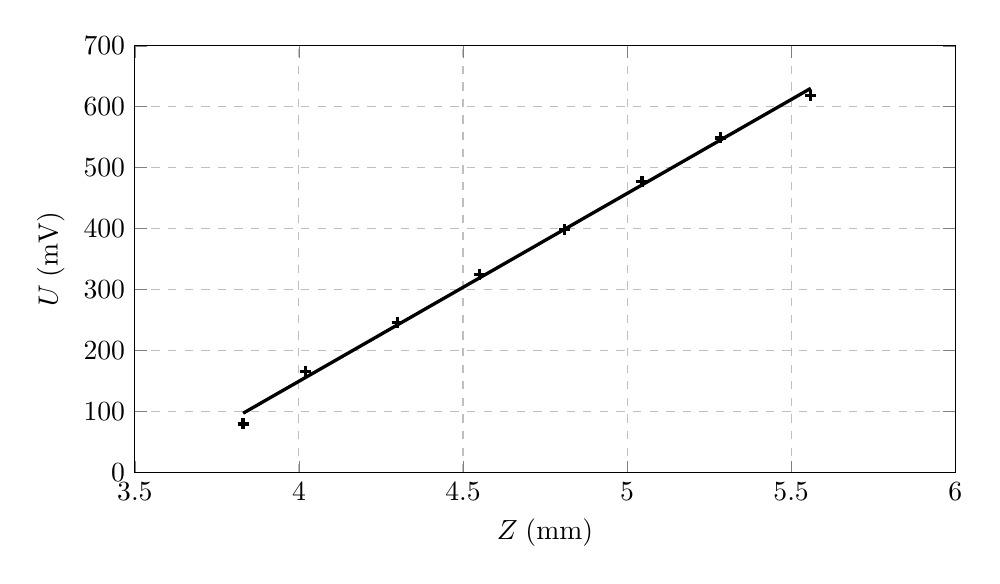
\begin{tikzpicture}
			\begin{axis}[
				legend pos=outer north east,
				width=12cm,height=7cm,
				xlabel=$ Z\;(\mathrm{mm}) $,
				ylabel=$ U\;(\mathrm{mV}) $,
				xmin=3.5,xmax=6,
				ymin=0,ymax=700,
				xtick={3.5,4,4.5,5,5.5,6},
				ytick={0,100,200,300,400,500,600,700},
				grid style=dashed,
				ymajorgrids=true,
				xmajorgrids=true,
				]
				\addplot[no marks,black,very thick] table[y={create col/linear regression={y=Y}}]
				{
					X	Y
					3.83	79.6
					4.019	165.7
					4.3 246
					4.55	325
					4.81	399
					5.045	477
					5.285	549
					5.56	619				
				};
				%\addlegendentry{
				%	$\pgfmathprintnumber{\pgfplotstableregressiona} \cdot x
				%	\pgfmathprintnumber[print sign]{\pgfplotstableregressionb}$}
				
				\addplot [very thick,mark=+,only marks] coordinates {
					(3.83,79.6)(4.019,165.7)(4.3,246)(4.55,325)
					(4.81,399)(5.045,477)(5.285,549)(5.56,619)
				};
			\end{axis}
		\end{tikzpicture}
		\caption{作图法计算霍尔位置传感器的灵敏度系数}
	\end{figure}

	取其中较远两点计算得斜率为$ 310.79\,\mathrm{mV/mm} $.
	
	\newpage
	
	~\
	
	\begin{center}
		\Large\bfseries 第三部分\quad 动态悬挂法测量材料的杨氏模量
	\end{center}
	\setcounter{section}{0}
	\section{实验目的}
	1.学会用动态悬挂法测量材料的杨氏模量;
	
	2.学习用外延法测量,处理实验数据;
	
	3.了解换能器的功能,熟悉测试仪器及示波器的使用;
	
	4.培养学生综合运用知识和使用常用实验仪器的能力。
	
	\section{实验器材}
	DHY-2A动态杨氏模量测试台,DH0803振动力学通用信号源,通用示波器、测试棒(铜、铝、不锈钢),悬线,专用连接导线,游标卡尺,螺旋测微器等。
	
	\section{实验原理}
	已知棒的横振动方程
	\[\frac{\mpar^4y}{\mpar x^4}-\frac{\rho S\mpar^2y}{YJ\mpar t^2}=0\]
	其中$ y $为棒振动的位移,$ Y $为杨氏模量,$ S $为棒的横截面积,$ J $为棒的转动惯量,$ \rho $为棒的密度,$ x $为位置坐标,$ t $为时间变量。
	
	用分离变量法对该方程进行求解,令$ y(x,t)=X(x)T(t) $,则有
	\[\frac1X\frac{\dif^4X}{\dif x^4}=\frac{\rho S}{YJ}\frac1T\frac{\dif^2T}{\dif t^2}\]
	要使上式成立,则左右两端需均等于一常数,不妨设该常数为$ K^4 $,则
	\[\frac{\dif^4X}{\dif x^4}-K^4X=0,\quad\frac{\dif^2 T}{\dif t^2}+\frac{K^4YJ}{\rho S}t=0\]
	求解以上两个方程可得通解
	\[y(x,t)=(A_1\cosh K_x+A_2\sinh K_x+B_1\cos K_x+B_2\sin K_x)\cos(\omega t+\varphi)\]
	其中$ \omega=\sqrt{\frac{K^4YJ}{\rho S}} $为频率公式,$ A_1,A_2,B_1,B_2,\varphi $是待定系数,可由边界条件和初始条件确定。
	
	对于长为$ L $,两端自由的棒,当悬线悬挂于棒的节点附近时,其边界条件为:自由端横向作用力、弯矩均为零,即
	\[F=-\frac{\mpar M}{\mpar x}=-EJ\frac{\mpar^3y}{\mpar x^3}=0,\quad M=EJ\frac{\mpar^2y}{\mpar x^2}=0\]
	即有
	\[\left.\frac{\dif^3X}{\dif x^3}\right|_{x=0}=\left.\frac{\dif^3X}{\dif x^3}\right|_{x=L}=\left.\frac{\dif^2X}{\dif x^2}\right|_{x=0}=\left.\frac{\dif^2X}{\dif x^2}\right|_{x=L}=0\]
	将其代入通解可得超越方程
	\[\cos KL\cdot\cosh KL=1\]
	该方程的解依次为0,\,4.7300,\,7.8532,\,10.9956,$\cdots$(此数列的值逐渐趋于$ K_nL=\frac{(n-1)\pi}{2} $)。
	
	上述第二个根$ K_1L=4.7300 $,与之相应的共振频率称为基频或固有频率$ \omega_1=2\pi f_1 $。
	
	对于直径$ d $,长为$ L $,质量为$ m $的圆形棒,其转动惯量为$ J=\frac{Sd^2}{16} $,在基频$ f_1 $下共振时,棒的杨氏弹性模量为
	\[Y=1.6067\frac{L^3mf_1^2}{d^4}\]
	测试棒在作基频振动时存在两个节点,它们的位置为距离端面$ 0.224L $处。理论上,悬挂点应取在节点处测试棒难以被激振和拾振,为此可在节点两端选用不同点对称悬挂,用外推法找出节点处的共振频率。
	
	此外,物体的固有频率$ f_{\text{固}} $与共振频率$ f_{\text{共}} $是两个不同的物理量,它们之间的关系为
	\[f_{\text{固}}=f_{\text{共}}\sqrt{1+\frac{1}{4Q^2}}\]
	其中$ Q $为测试的机械品质因素。应用悬挂法测量时,一般$ Q $的最小值约为50,此时共振频率与固有频率相比仅差0.005\%。本实验中仅能测出共振频率,可利用两者间相差很小用共振频率代替固有频率。
	
	\section{实验内容}
	1.测量测试棒的长度$ L $,直径$ d $,质量$ m $\footnote{质量$ m $由实验室提供},为提高测试精度,以上量均需测量3次;
	
	2.测量测试棒在室温时的共振频率$ f_1 $:
	
	\tab\tab (1)安装测试棒:将测试棒悬挂于两悬线上,要求测试棒横向水平,悬线于测试棒轴向垂直,两悬线挂点到测试棒两端点的距离分别为$ 0.0365L $和$ 0.9635L $处,并处于静止状态;
	
	\tab\tab (2)连机:将测试台、信号源、示波器之间用专用导线连接;
	
	\tab\tab (3)开机:分别打开示波器、信号源的电源开关,调整示波器处于正常工作状态;
	
	\tab\tab (4)鉴频与测量:待测试棒稳定后,调节信号频率与幅度,寻找测试棒的共振频率$ f_1 $。当示波器荧光屏上出现共振现象(正弦波振幅突然变大)时,十分缓慢地微调频率调节细调旋钮,使得波形振幅达到极大值。容易发现测试棒不只在一个频率处发生共振现象,需确认测试棒是在基频频率下共振。这就是鉴频过程。
	
	测量完成$ 0.0365L,\;0.9635L $处后,再分别按$ 0.099L,\;0.901L $一组,$ 0.1615L,\;0.8385L $一组,$ 0.224L,\;0.776L $一组,$ 0.2865L,\;0.7135L $一组,$ 0.349L,\;0.651L $一组,$ 0.415L,\;0.585L $一组进行测量。
	
	\section{实验结果与数据处理}
	1.铜金属棒的质量由实验室给出:$ m=42.121\,\mathrm g $,其长度$ L $与直径$ d $:
	\begin{table}[!h]
		\centering
		%\renewcommand\arraystretch{}
		\begin{tabularx}{\textwidth}{|c|Y|Y|Y|Y|}
			\hline
			\textbf{测量次数}&\textbf{1}&\textbf{2}&\textbf{3}&\textbf{平均值}\\
			\hline
			\textbf{长度$ \bm L $(mm)}&180.4&180.3&180.3&180.33\\
			\hline
			\textbf{直径$ \bm d $(mm)}&5.953&5.961&5.960&5.958\\
			\hline
		\end{tabularx}
		\caption{铜金属棒几何尺寸测量}
	\end{table}

	2.铜金属棒处于不同悬挂位置处时的共振频率为
	\begin{table}[!h]
		\centering
		%\renewcommand\arraystretch{1.1}
		\begin{tabularx}{\textwidth}{|c|Y|Y|Y|Y|Y|Y|Y|}
			\hline
			\textbf{序号}&\textbf{1}&\textbf{2}&\textbf{3}&\textbf{4}&\textbf{5}&\textbf{6}&\textbf{7}\\
			\hline
			\textbf{悬挂点位置$ x\,\mathrm{(mm)} $}&6.57&17.82&29.07&40.32&51.57&62.82&81.27\\
			\hline
			\textbf{共振频率$ {f}\,(\mathrm{Hz}) $}&603.3&594.7&588.1&无&587.6&590.3&595.0\\
			\hline
		\end{tabularx}
		\caption{铜金属棒在不同悬挂位置下的共振频率}
	\end{table}

	3.根据上表可画出如下$ x-f $图象:
	\begin{figure}[!h]
		\centering
		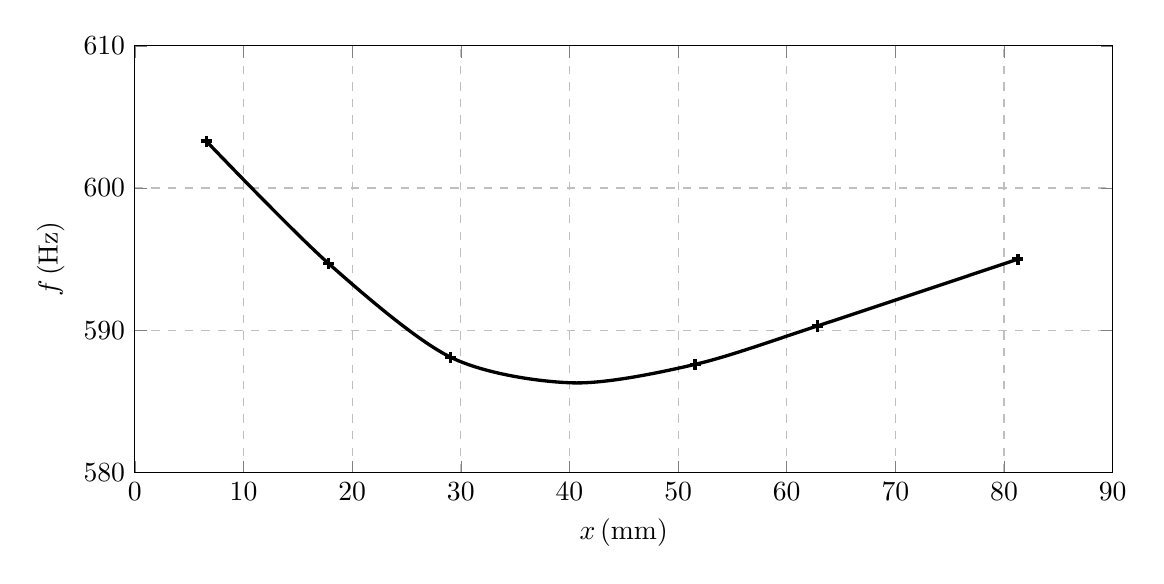
\begin{tikzpicture}
			\begin{axis}[
				xlabel=$ x\,\mathrm{(mm)} $,
				ylabel=$ f\,\mathrm{(Hz)} $,
				width=14cm,height=7cm,
				xmin=0,xmax=90,
				ymin=580,ymax=610,
				xtick={0,10,20,30,40,50,60,70,80,90},
				ytick={580,590,600,610},
				grid style=dashed,
				ymajorgrids=true,
				xmajorgrids=true,
				]
				\addplot [very thick,no marks,smooth] coordinates {
					(6.57,603.3)(17.82,594.7)(29.07,588.1)
					(40.32,586.3)
					(51.57,587.6)(62.82,590.3)(81.27,595.0)
				};
				
				\addplot [very thick,mark=+,only marks] coordinates {
					(6.57,603.3)(17.82,594.7)(29.07,588.1)
					(51.57,587.6)(62.82,590.3)(81.27,595.0)
				};
			\end{axis}
		\end{tikzpicture}
		\caption{铜金属棒的悬挂位置与相应共振频率关系曲线图}
	\end{figure}
	
	由上图平滑曲线可读得$ x=40.32\,\mathrm{mm} $处的共振频率$ f_1=f=586.3\,\mathrm{Hz} $,代入杨氏模量计算公式可得
	\[Y=1.6067\frac{L^3mf_1^2}{d^4}=1.082\times10^{11}\,\mathrm{N/m^2}\]
	
	\newpage
	
	~\
	
	\begin{center}
		\Large\bfseries 第四部分\quad 思考题与实验总结
	\end{center}
	\setcounter{section}{0}
	\section{思考题}
	1.杨氏模量测量数据$ N $若不用逐差法而用作图法,应当如何处理?
	
	{\kaishu 根据数据的取值范围合理标定坐标轴,在坐标系中描出实验中测得的数据点,根据数据点的分布画出一条拟合直线穿过这些点,使得数据点尽量均匀地落在直线两侧,在拟合直线上取相距较远地两点,读出坐标值计算的得到直线的斜率,得到最终结果。}
	
	~\
	
	2.两个材料相同但粗细不同的金属丝,它们的杨氏模量相同吗?为什么?
	
	{\kaishu 相同。杨氏模量是描述固体材料本身抵抗形变能力的物理量,仅取决于材料的物理性质,而与其规格、形状均无关。}
	
	~\
	
	3.本实验使用了哪些测量长度的量具?选择它们的依据是什么?它们的仪器误差各是多少?
	
	{\kaishu 本次实验所用测量长度的量具、相应指标与作为例子选取的几个这些仪器分别适合测量的物理量小结如下表。选择依据为量程满足对待测长度的测量,精度符合实验需要。}
	
	\begin{table}[!h]
		\centering
		\renewcommand\arraystretch{1.5}
		\begin{tabularx}{\textwidth}{|c|Y|Y|Y|c|c|}
			\hline
			\textbf{仪器名称} & \textbf{分度值$ \bm d $} & \textbf{量程} &\textbf{允差$ \bm e $}& \textbf{仪器特点} & \textbf{测量的物理量(例)}\\
			\hline
			螺旋测微器 & 0.01\,mm & 25\,mm &$ \pm0.004\,\mathrm{mm} $& {\small 量程小而精度高} & {\small 钼丝直径、黄铜横梁厚度}\\
			\hline
			钢卷尺 & 1\,mm & 3\,m &$ \pm 2.0\,\mathrm{mm} $& {\small 量程大而精度小} & {\small 钼丝长度}\\
			\hline
			游标卡尺 & 0.02\,mm & 20\,cm &$ \pm0.02\,\mathrm{mm} $& {\small 量程大而精度高} & {\small 黄铜横梁宽度}\\
			\hline
			钢板尺 & 1\,mm & 30\,cm &$ \pm0.12\,\mathrm{mm} $& {\small 测量易而精度中} & {\small 黄铜横梁刀口距离}\\
			\hline
		\end{tabularx}
		\caption{实验所用长度测量量具}
	\end{table}
	
	4.在CCD法测定金属丝杨氏模量实验中,为什么起始时要加一定数量的底码?
	
	{\kaishu 初始状态下金属丝都可能有一定程度的弯曲,通过加上一定的底码可以拉直钼丝,既避免钼丝产生轴向伸缩形变以外的形变,也能使得测得钼丝的长度更为准确。}
	
	~\
	
	5.加砝码后标示横线在屏幕上可能上下颤动不停,不能够完全稳定时,如何判定正确读数?
	
	{\kaishu 等待其振动幅度减小至一定程度,振动可近似看作简谐振动后,取读数的极大值、极小值,计算平均值作为最终读数。}
	
	~\
	
	6.弯曲法测量杨氏模量实验,主要误差有哪些?请估算各因素的不确定度。
	
	{\kaishu 根据弯曲法测杨氏模量的原理公式(\ref{2}),可能的误差来源有:黄铜片的几何尺寸(厚度$ a $、宽度$ b $、长度$ d $)、加力系统示数的跳变等。前者的不确定度见公式(6,7,8),后者通常等待示数稳定后读数,故而不确定度可认为为$ u(M)=0.1\,\mathrm g $(即分度值)。}
	
	~\
	
	7.用霍尔位置传感器测位移有什么优点?
	
	{\kaishu 霍尔位置传感器在测量位移的灵敏度上较高,同时以电信号的形式输出位移信息,免去了估读等工作,简化了实验步骤。}
	
	~\
	
	8.请自行分析实验过程中和数据分析时遇到的问题,找到处理的方法。
	
	{\fangsong 问题1:数据处理过程中有时计算结果与理论值间出现数个数量级间的差距。}
	
	{\kaishu 解决方案:该问题通常来自物理量单位间的换算,可检查公式中各物理量代入时的单位是否统一、换算是否正确。}
	
	{\fangsong 问题2:弯曲法测杨氏模量中,显微镜示数数据记录起初仅根据视野内刻度,得到数据精度仅为$ 0.1\,\mathrm{mm} $,明显在精度上不足。}
	
	{\kaishu 解决方案:该问题来自于对实验内容的预习不足,读数显微镜的测量结果除视野中的毫米刻度线外还有上方的鼓轮读数。鼓轮的读数方式与螺旋测微器类似。}
	
	\section{实验反思与心得体会}
	在我个人的实验顺序中,本次实验是第一个力学实验\footnote{此前的四个正式实验为电磁学、光学实验};而按照实验讲义的顺序,本次实验是第一个正式实验。在实际实验与数据处理的过程中,我认识到了许多在此前实验中不曾用心了解过的内容,如减小实验误差的手段、不确定度的计算、不同的数据处理方法。虽然在数据处理上繁琐,但本次实验在实验习惯、思维上的启迪对后续实验相信都有着深远的影响,这样也不难理解为何要将其安排为“第一个”正式实验。
\end{document}